\documentclass[11pt]{article}

\usepackage{fullpage}
\usepackage{enumerate}
\usepackage{natbib}
\usepackage{graphicx}
\usepackage{hyperref}
\usepackage{ifthen}
\usepackage[all]{hypcap}
\newcommand{\logfig}[2]{
See figure~\ref{fig:#1}.
\begin{figure}[!ht] 
\includegraphics[width=0.9\textwidth]{#1} 
\caption{#2} 
\label{fig:#1} 
\end{figure}
}

\bibliographystyle{aa_arxiv}

\title{Analysis Document: Weak Lensing Calibration with N-body Simulations}
\date{Started ~Feb 2013}
\author{Douglas Applegate}


\begin{document}

\maketitle

\tableofcontents

%%%%%%%%%%%%%%%%%%%%%%%%%%%%%%%%%%%%%%%%%%%%%%%%%%%%%%%%%%%%%

\section{Project Description}

The goal of this project is to measure and improve the systematic uncertainty from mass-profile modeling in weak lensing. In the Weighing the Giants analysis, we assumed an NFW density profile. Does that bias the mean mass of the sample? How well can we constrain that bias? Starting at that point, I am to answer some of the following questions:

\begin{itemize}
\item What is the bias when you fit an NFW halo? What is the optimal radial range to fit, in terms of bias, systematic uncertainty and statistical uncertainty?
\item Is the NFW profile the best description? Do other profiles work better? Are there other ways to measure masses (eg Mass Aperture) that are better?
\item How does this evolve with cluster mass, and with redshift? Are there other predictors?
\item How do we best handle the mass-concentration relation?
\item How do we best handle the prior on cluster mass?
\item Are there differences in predictions from different simulations, and from different ways to simulate lensing?
\end{itemize}

The simulations may also give insights into more advanced topics, such as 
\begin{itemize}
\item What can simulations tell us about applying contamination corrections?
\item Can we measure cluster concentrations?
\item Can we measure cluster ellipticities, and over what radial range?
\item If designing a survey from scratch, how should we do it?
\end{itemize}

There are currently three analysis efforts that these results feed into. The first is the Stanford Weighing the Giants work, with Steve, Adam, and Anja, working with wide field, ground-based observations from Subaru. Then there is the SPT efforts at low and high redshifts, with Tim and Joerg. The high-z work uses HST observations, whereas the low-z work uses Megacam @ Magellan. Finally, this work also feeds into the LSST effort.


%%%%%%%%%%%%%%%%%%%%%%%%%%%%%%%%%%%%%%%%%%%%%%%%%%%%%%%%%%%%%

\section{Log}

\paragraph{15 July 2013}
Lots of development work during the March period that was undocumented. 
Basically, got running on Becker's simulations. 
Oddly, though, I couldn't reproduce his results. 
Not sure why, but it may be because I am only looking at the most massive halos while he was fitting biases to all halos.
While there are many things that I can do to try to recover Matt's results, I don't know if I can.
First step is to go back to my results, and just figure out what is going on.


\paragraph{01 Jan 2013}
Start of this work package. 
First step is to clean up old code that I've been using in bonnpipeline and get it running with Will's simulated catalogs.

\paragraph{06 Aug 2013}
I've recieved from Jiayi in Munich a distribution of SZ - halo center offsets from a new set of hydro sims they've done. I'm going to explore the offset distributions and effects on an NFW halo in an ipython notebook called: simulated\_offsets.ipynb .

\paragraph{19 Feb 2014}
After a long gap in this notebook, I'm back to updating it and tracking my research investigations. Since I've last updated, I've added two new simulation sets, the BCC and the MXXL. I've implemented a uniform analysis, and have begun exploring different radial ranges, as well as differences between the two simulations. I've updated all sections of the notebook to try to capture these pieces.


%%%%%%%%%%%%%%%%%%%%%%%%%%%%%%%%%%%%%%%%%%%%

\section{Guide to Files \& Software}

TODO: Fill in guide to software



%%%%%%%%%%%%%%%%%%%%%%%%%%%%%%%%%%%%%%%%%%%%%%%%%%%%%%%%%%%%%

\section{Available Simulations}

I have access to 3 sets of simulations:

\paragraph{BK11} : Cut-outs around massive halos at redshifts z=0.25 and z=0.5, used in Becker \& Kravtsov 2011. Particles are extracted in a 20x20x400 comoving Mpc/h box around each cluster and are projected to form a 2-D mass map. From that, a shear signal is calculated, assuming sources are at z=1

\paragraph{BCC} : A simulation of a large sky-area survey covering a continuous patch of sky. Three boxes of decreasing resolution are appended and are used to form a past light cone of the visible universe. The simulation ray-traces shear from each galaxy in the simulation to the observer at z=0. I have extracted galaxies centered around the lensed central position of each massive halo in the simulation. From Wechsler, Becker, and Buscha, priv comm.

\paragraph{MXXL}: A large box where snapshots at particular redshifts are written to disk. I currently have only the z=1 snapshot. Sources are assumed to be at infinite distance (not infinite redshift). Shear is calculated by projecting masses to a plane in a box (of unknown size) around each massive cluster. I have 3 projections for each cluster.


%%%%%%%%%%%%%%%%%%%%%%%%%%%%%%%%%%%%%%%%%%%%%%%%%%%%%%%%%%%%%

\section{Are the simulations consistent?}

In the most basic test, do I recover the same bias as a function of mass from each simulation? There are a few reasons why I might not. 

\begin{itemize}
\item Each simulation probes a different redshift range, so I should be able to probe redshift evolution. Thankfully, the BCC bridges between the MXXL and BK11, while I will also hopefully receive additional snapshots from the MXXL. 
\item Each simulation uses a slightly different cosmology. That may mean that the mass-concentration relations are different, which may again lead to different biases. 
\item Each simulation is at different resolutions, so there could be resolution issues, especially near the cluster centers. 
\item The BCC ray traces over a past light cone, whereas BK11 and the MXXL ignore LSS evolution and don't ray trace
\item The density of points where the shear field is measured is different. Bahe+2012 shows that lower density surveys / noisier surveys average over / miss some substructure, leading to different bias results.
\item There may be a bug in how I'm reading in one of the simulations. This was previously a problem with the BK11 simulations, where I first missed factors of h, and then there was ambiguity about at what redshift the lensing signal was calculated for.
\end{itemize}

\subsection{Basic Analysis Approach}

TODO: Fill in details here on how exactly I do my fits.

The fit is encoded in nfwfit.py. 


\subsection{Comparing Mass Bias vs Radial Range \& M-C Relation}
\label{sec:consistant_bias_mcrelation}

I've run mass fits with three mass-concentration relations: c=4, the Duffy08 relation, and allowing c to be fit freely.

I've run fits for 15 different radial ranges: 3 Inner radii {0.25, 0.5, 0.75 Mpc}, and 6 outer radii {0.5, 0.75, 1.0, 1.5, 2.5, 3.0}. The radial ranges are encoded as follows:

\begin{itemize}
\item 'r1' : '0.25 - 0.5 Mpc',
\item 'r2' : '0.25 - 1.5 Mpc',
\item 'r3' : '0.25 - 2.5 Mpc',
\item 'r4' : '0.25 - 3.0 Mpc',
\item 'r5' : '0.50 - 1.5 Mpc',
\item 'r6' : '0.50 - 2.5 Mpc',
\item 'r7' : '0.50 - 3.0 Mpc',
\item 'r8' : '0.75 - 1.5 Mpc',
\item 'r9' : '0.75 - 2.5 Mpc',
\item 'r10' :'0.75 - 3.0 Mpc',
\item 'r11' :'0.25 - 0.75 Mpc',
\item 'r12' :'0.25 - 1.0 Mpc',
\item 'r13' :'0.50 - 0.75 Mpc',
\item 'r14' :'0.50 - 1.0 Mpc',
\item 'r15' :'0.75 - 1.0 Mpc'
\end{itemize}


When I assume either c=4 or Duffy08, I see that the simulations produce different results. The slopes of bias vs mass change, as well as the absolute normalizations. The three simulations appear to respond differently as well. See figure~\ref{fig:comparing_r7_bias}. The curves seem to shift some between simulations. But since I am refitting the same halos, I would expect that the shifts in each simulation are real. Only when I go to cfree are the BCC and MXXL seemingly consistent. BK11 is hanging out by itself for some reason, which I don't understand.

\begin{figure}[!ht]
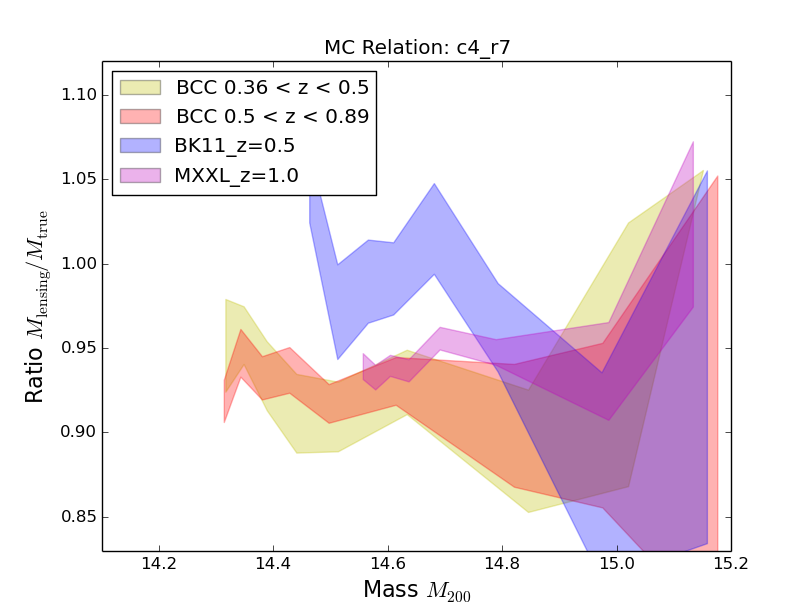
\includegraphics[width=0.25\textwidth]{figures/c4_r7}
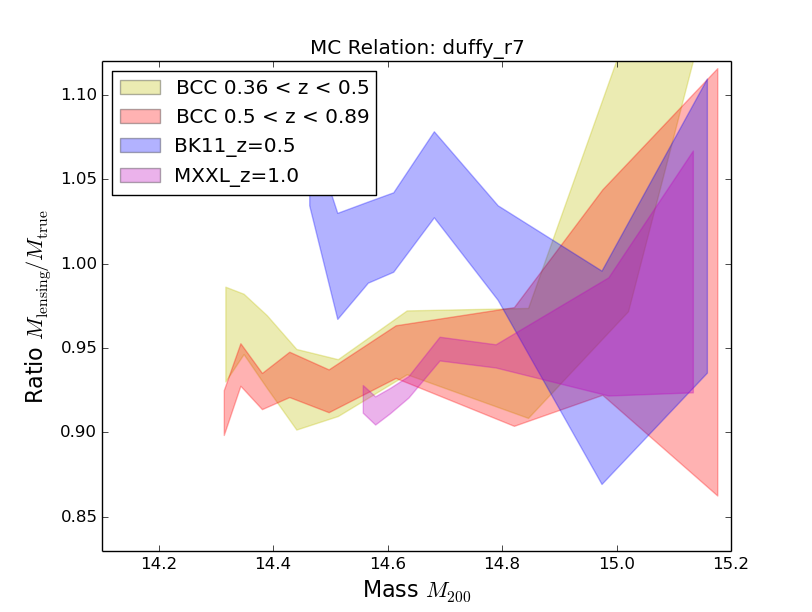
\includegraphics[width=0.25\textwidth]{figures/duffy_r7}
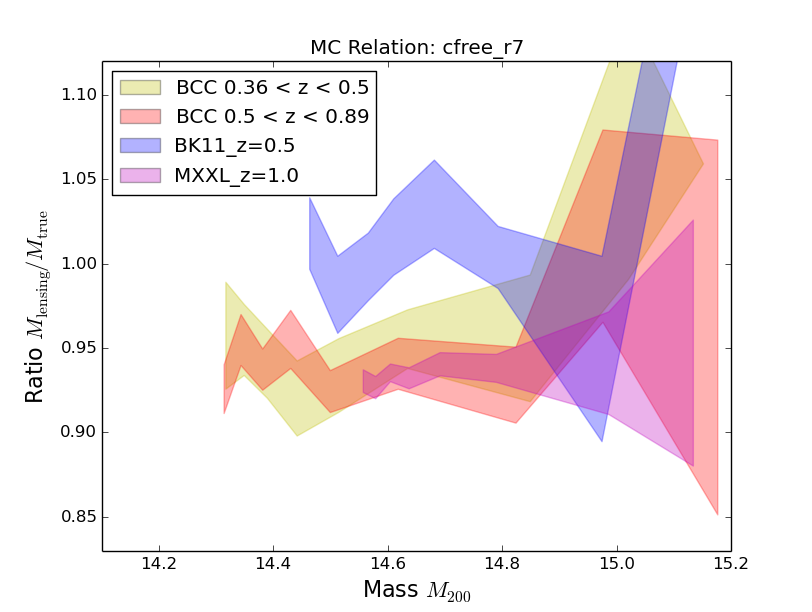
\includegraphics[width=0.25\textwidth]{figures/cfree_r7}
\caption{Plot of bias versus mass. Left: Assuming c=4, Center: Assuming Duffy08, and Right: C is a free parameter. The fit range is 0.5 - 3.0 Mpc. The width of each colored band represents the $1\sigma$ uncertainty in the median bias for each mass bin. Bins are adaptively created to balance signal-to-noise with exploring the mass range. Made with compareDiffSims.py}
\label{fig:comparing_r7_bias}
\end{figure}

The agreement between BCC and MXXL seems to be fit range dependent. The above fits covered a range of 0.5 - 3.0 Mpc. If we only look at the outer region for cfree, the fits are again good.

\logfig{figures/cfree_r10}{Same as fig~\ref{fig:comparing_r7_bias}, except now only for cfree and 0.75-3Mpc.}

However, if we look at the innermost fit region, 0.25-0.5 mpc, we can see that the two simulations are drastically different. BCC and BK11 show diving calibrations at the high mass end (0.2 for $10^{15}$ halos!?), but MXXL holds relatively steady up to the highest masses. 

\logfig{figures/cfree_r1}{Same as fig~\ref{fig:figures/cfree_r10}, except for on a radically different scale.}

Could this be a resolution effect? Or maybe how the shear signal is calculated, since we are getting close to the critical curves, though I would think if that was the case BK11 and MXXL would be more consistent. We also should only be seeing shears of $g\approx0.3$ at 250kpc for z=1 and $10^{15}$ solar masses.


\subsection{Role of Mass-Concentration Relation}

I think that the behavior of the fits against the different mass-concentration relations vs cfree suggests that the simulations have intrinsically different m-c relations. This is supported by the work of \citet{ludlow_mc}, which shows that even for $M_{200} = 10^{14}$ clusters, the mean concentration can vary by 20\% over the WMAP1-7 and Planck cosmologies. 

This to me suggests a 2-pronged strategy. When we don't care about cosmology, for example, just talking about masses, then we can fix a mass-concentration relation (appropriate for that cosmology). However, for purposes of cosmological fits, we need to vary the m-c relation systematically over all clusters inline with the fit. That way we don't get hit by some ``systematic uncertainty'' by assuming an M-C relation, and we capture the covariance with cosmology.


\subsection{Next Steps}

\begin{itemize}
\item I want to stack cluster shear profiles (grouping by mass, redshift, and concentration), and see if I can visually see differences at low redshifts. Maybe I should stack residuals? That might confirm my suspicion that there is some sort of different treatment or resolution effect afflicting cluster cores in BCC and BK11.
\item I should implement the Ludlow prescription for cosmology-dependent m-c relations. I should then check to see if I get a consistant bias across all three simulations/cosmologies. That would confirm my suspicion about how to treat the m-c relation, while being robust to non-consenus parameter values.
\end{itemize}


%%%%%%%%%%%%%%%%%%%%%%%%%%%%%%%%%%%%%%%%%%%%%%%%%%%%%%%%%%%%%

\section{Optimal Radial Ranges for NFW Profiles}

Question: What is the best radial range to use when fitting an NFW profile? I need to provide answers in two different regiemes, which in the end may end up overlapping. The first is the SPT regime, where the limited field of view on Hubble restricts how far out we can probe. The second regime is ground-based wide-field data from Subaru or LSST, where we can go out as far as we want.

I ran 15 different fit ranges (see~\ref{sec:consistant_bias_mcrelation}) for all 3 simulations. Right now I am biased towards MXXL, so I will only show results for that at the moment.

\logfig{figures/cfree}{Plotting mass bias from lensing versus cluster mass, using the MXXL simulation and no m-c relation, for different radial ranges. Line styles denote different inner fit boundaries, while color denotes different outer fit boundaries. Color are grouped, suggesting that the outer fit boundary is more important than the inner fit boundary. Produced with compareSims.py}

Outer fit range seems to matter much more than inner fit range. You might expect that the behavior changes as the fit includes or excludes r200. R200 is at ~1.1Mpc for $10^{14.5}$ clusters, whereas it is closer to 1.4Mpc for $10^{15}$ clusters. So for example, fitting out to 1Mpc is inside R200 for all clusters, and that bias seems to stay pretty level for all masses (the last bin is noisy). The pink line, fitting to 1.5mpc, is somewhat outside R200 for the lighter clusters, and just barely outside for the most massive -- that line shows larger cluster masses at higher true masses. If for some reason fitting m\&c biases masses up, then the pink line could be converging to the ``right'' answer at higher masses. Similar story for 2.5 and 3 Mpc, where masses are notably underestimated at low masses, and the trend heads to less bias at higher masses. I'm not sure how to explain the green lines, fitting to only 750kpc. 


\textbf{Could I fit perfect NFW halos and add noise? That way I could see the effects of noise bias on a two parameter fit?}


\logfig{figures/cfree_scatter}{Plotting intrinsic scatter versus mass for different radial ranges, using the MXXL simulation and no m-c relation. Same coloring and line scheme as fig.~\ref{fig:figures/cfree}. Scatter increases as I limit the outer radius used in the fit.}

The story with the scatter is much clearer. As I move the outer radial range to small values, the amount of scatter picks up. As soon as I move inside R200, the scatter blows up. Why is this? Smaller area, so subject to more LSS noise? More substructure in clusters?

\subsection{Next Steps}

For the HST proposal (due to STSCI in April, but need it for proposal writing by 25 Feb 2014), I need to add shape noise, use a lower sampling density, and apply HST masks associated with our mosaicing programs. That way I can directly measure the expected scatter for different choices, which will affect how powerful the HST program will be. 

There are some more general steps that I would like to do as well:
\begin{itemize}
\item Noise. I want to understand how the 2-parameter fit responds to noise. I could create perfect NFW halos and add shape noise to see how the best fit value changes. I also want to explore the 2D posterior surface for some of the clusters in MXXL, both relaxed and unrelaxed. Related, how does the posterior perform when I marginalize over it instead of using a point estimator?
\item We may in the end use a 1-parameter fit, but since the M-C relation is cosmology dependent, I need to implement a cosmology dependent relation. How does that perform?
\end{itemize}

%%%%%%%%%%%%%%%%%%%%%%%%%%%%%%%%%%%%%%%%%%%%

\section{What is the best mass to measure?}

The above work was done looking at M200. However, as it currently stands, we are calibrating masses closer to M500. There is also an open question as to what mass is the least sensitive to m-c assumptions, or put another way, what is the mass that lensing measures the best?

To start, I'd like to remake the above plots with M500 instead of M200. However:

\begin{itemize}
\item The BCC M500 values appear to be larger than the M200 values
\item The MXXL M500 values that I have are for the z=0 slice, not the z=1 slice.
\end{itemize}

I've contacted Aaron about the MXXL problem, but I am holding off contacing Matt about the BCC issue until I am ready to show him some preliminary results.



%%%%%%%%%%%%%%%%%%%%%%%%%%%%%%%%%%%%%%%%%%%%%%%%%%%%%%%%%%%%%%


\section{Collaborators, Acknowledgements, Debts}

\subsection{Collaborators}

Stanford
\begin{itemize}
\item Steve Allen
\item Anja von der Linden
\item Pat Kelly
\item Adam Mantz
\item Glenn Morris
\end{itemize}

Bonn
\begin{itemize}
\item Tim Schrabback
\item Peter Schneider
\end{itemize}

SPT
\begin{itemize}
\item Brad Benson
\item Joerg Dietrich
\end{itemize}

MXXL Simulations
\begin{itemize}
\item Stefan Hilbert
\end{itemize}

BCC Simulations
\begin{itemize}
\item Risa Wechsler
\item Matt Becker
\item Michael Buscha
\end{itemize}

BK11 Simulations
\begin{itemize}
\item Matt Becker
\end{itemize}


%%%%%%%%%%%%%%%%%%%%%%%%%%%%

\bibliography{refs.bib}

%%%%%%%%%%%%%%%%%%%%%%%%%%%%%



\end{document}

